\documentclass[preprint]{elsarticle}
\usepackage{amsmath}
\usepackage{tikz}
\usetikzlibrary{shapes,decorations.pathmorphing,decorations.markings}

\begin{document}

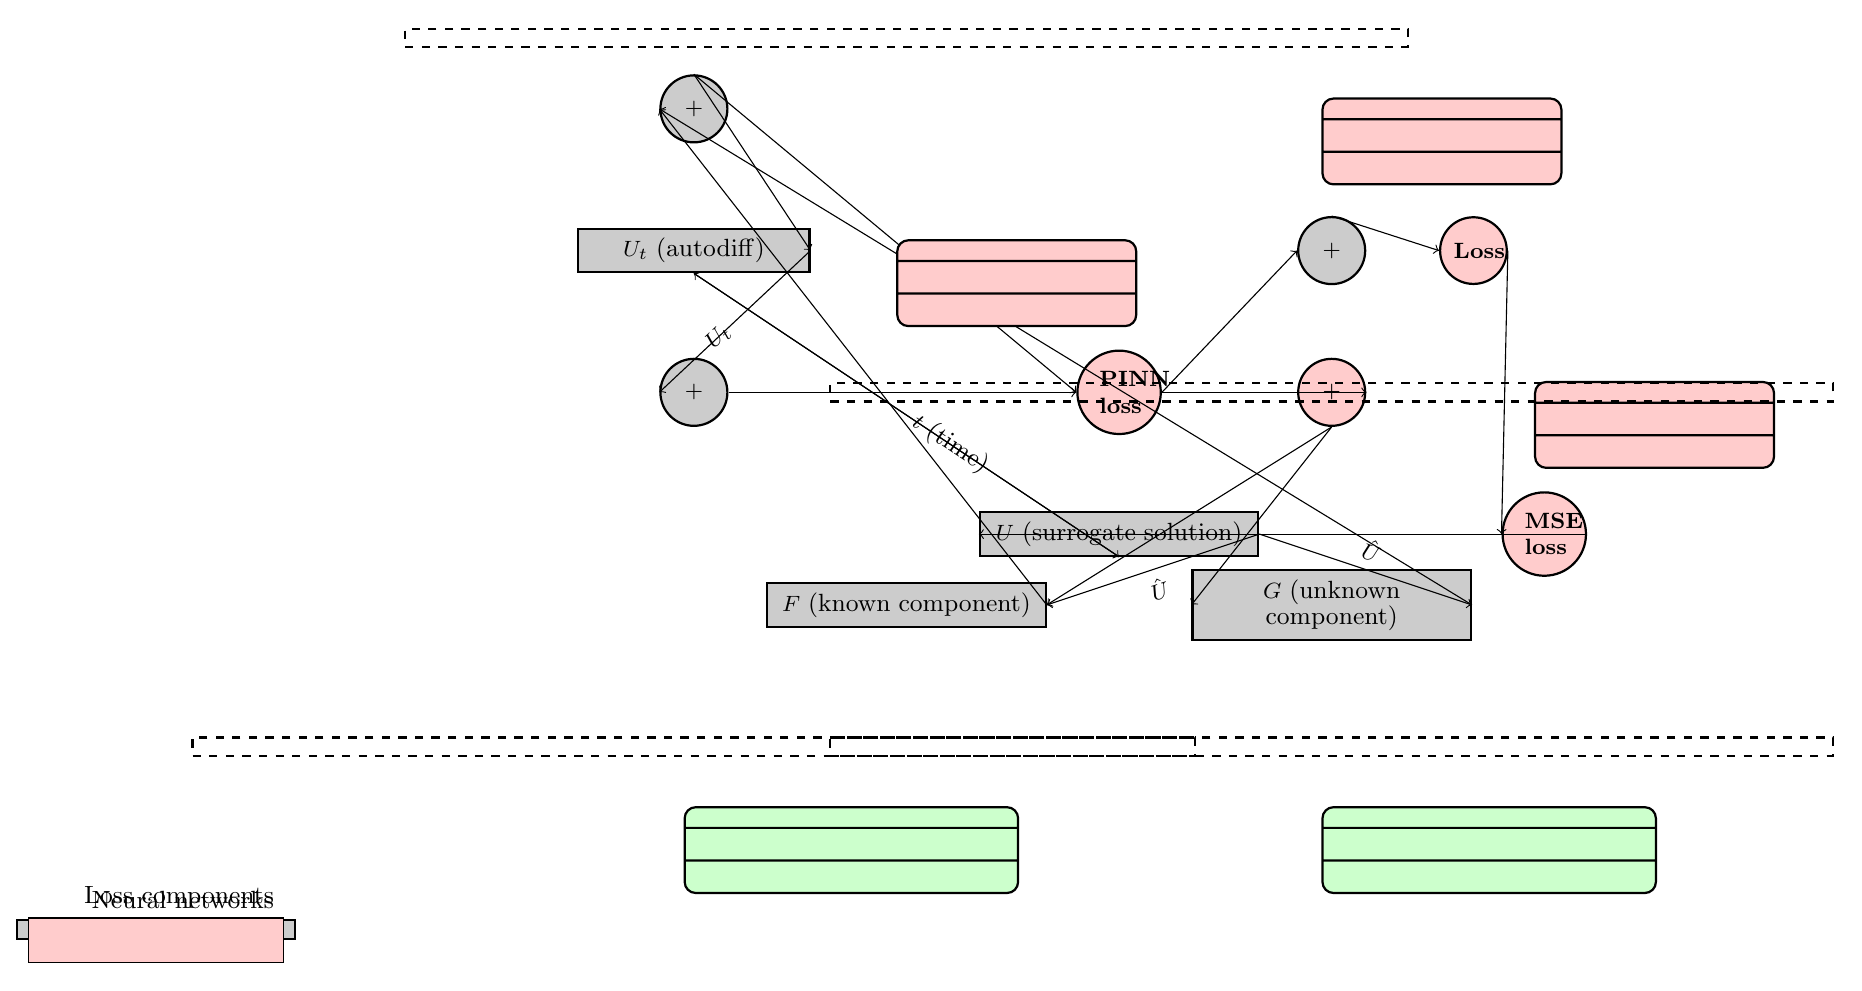
\begin{tikzpicture}[font=\footnotesize,scale=0.9]
	\node[circle,draw=black,fill=red!20,thick,text width=0.5cm,align=center] (loss) at (8,4) {\textbf{Loss}};
	\node[circle,draw=black,fill=red!20,thick,text width=0.5cm,align=center] (PINN) at (3,2) {\textbf{PINN loss}};
	\node[circle,draw=black,fill=red!20,thick,text width=0.5cm,align=center] (mse) at (9,0) {\textbf{MSE loss}};
	\node[circle,draw=black,fill=red!20,thick,text width=0.5cm,align=center] (plus) at (6,2) {+};
	\node[rectangle,draw=black,fill=black!20,thick,text width=3.3cm,align=center] (U) at (3,0) {$U$ \small{(surrogate solution)}};
	\node[rectangle,draw=black,fill=black!20,thick,text width=3.3cm,align=center] (F) at (0,-1) {$F$ \small{(known component)}};
	\node[rectangle,draw=black,fill=black!20,thick,text width=3.3cm,align=center] (G) at (6,-1) {$G$ \small{(unknown component)}};
	\node[circle,draw=black,fill=black!20,thick,text width=0.5cm,align=center] (plus2) at (-3,2) {+};
	\node[rectangle,draw=black,fill=black!20,thick,text width=2.7cm,align=center] (UT) at (-3,4) {$U_t$ \small{(autodiff)}};
	\node[circle,draw=black,fill=black!20,thick,text width=0.5cm,align=center] (plus3) at (-3,6) {+};
	\node[circle,draw=black,fill=black!20,thick,text width=0.5cm,align=center] (plus4) at (6,4) {+};
	
	\draw[->] (UT.east) -- node[pos=0.5,left,sloped] {$U_t$} (plus2.west);
	\draw[->] (plus2.east) -- node[pos=0.5,above,sloped] {} (PINN.west);
	\draw[->] (PINN.east) -- node[pos=0.5,right,sloped] {} (plus.east);
	\draw[->] (plus.south) -- node[pos=0.5,above,sloped] {} (F.east);
	\draw[->] (plus.south) -- node[pos=0.5,below,sloped] {} (G.west);
	\draw[->] (G.east) -- node[pos=0.5,above,sloped] {} (plus3.west);
	\draw[->] (F.east) -- node[pos=0.5,below,sloped] {} (plus3.west);
	\draw[->] (plus3.north) -- node[pos=0.5,right,sloped] {} (PINN.west);
	\draw[->] (plus3.north) -- node[pos=0.5,left,sloped] {} (UT.east);
	\draw[->] (PINN.east) -- node[pos=0.5,right,sloped] {} (plus4.west);
	\draw[->] (plus4.north) -- node[pos=0.5,right,sloped] {} (loss.west);
	\draw[->] (loss.east) -- node[pos=0.5,left,sloped] {} (mse.west);
	\draw[->] (mse.east) -- node[pos=0.5,right,sloped] {} (U.west);
	\draw[->] (U.east) -- node[pos=0.5,above,sloped] {$\hat{U}$} (G.east);
	\draw[->] (U.east) -- node[pos=0.5,below,sloped] {$\hat{U}$} (F.east);
	\draw[->] (U.south) -- node[pos=0.5,right,sloped] {$t$ \small{(time)}} (UT.south);
	\draw[->] (UT.south) -- node[pos=0.5,below,sloped] {} (U.south);
	
	\begin{scope}[every node/.style={draw, rounded corners}]
		\node[rectangle split,rectangle split parts=3,fill=green!20,thick,text width=4cm,align=center,anchor=text] at (6,-4){};
		\node[rectangle split,rectangle split parts=3,fill=green!20,thick,text width=4cm,align=center,anchor=text] at (-3,-4){};
		\node[rectangle split,rectangle split parts=3,fill=red!20,thick,text width=2.8cm,align=center,anchor=text] at (0,4){};
		\node[rectangle split,rectangle split parts=3,fill=red!20,thick,text width=2.8cm,align=center,anchor=text] at (6,6){};
		\node[rectangle split,rectangle split parts=3,fill=red!20,thick,text width=2.8cm,align=center,anchor=text] at (9,2){};
	\end{scope}
	\node[draw,dashed,fill=none,thick,text width=12.5cm,align=center,anchor=center] at (-3,-3) {};
	\node[draw,dashed,fill=none,thick,text width=12.5cm,align=center,anchor=center] at (6,-3) {};
	\node[draw,dashed,fill=none,thick,text width=12.5cm,align=center,anchor=center] at (0,7) {};
	\node[draw,dashed,fill=none,thick,text width=12.5cm,align=center,anchor=center] at (6,2) {};
	
	\path[overlay,draw=black]
	(current bounding box.south west)+(-0.5,-0.5) node[rectangle,draw=black,fill=black!20,thick,text width=3.3cm,align=center] (legend) {};
	\draw[draw=black, fill=green!20] ([xshift=5pt,yshift=-0.5pt]legend.south west) rectangle ([xshift=-5pt,yshift=0.5pt]legend.north east) node[anchor=south east] {\small Neural networks};
	\draw[draw=black, fill=red!20] ([xshift=5pt,yshift=-0.5pt]legend.south west)+(0,-2ex) rectangle ([xshift=-5pt,yshift=0.5pt]legend.north east) node[anchor=south east] {\small Loss components};
\end{tikzpicture}

\end{document}